\label{ch:symmetry}

\section{Cayley diagram}
\label{sec:cayley-diagram}

We have seen in the previous chapter how cyclic groups
(those generated by a single generator)
have neatly described torsors.

In this section we shall generalize this story
to groups $G$ generated by a
(finite or just decidable)
set of generators $S$.

\tikzset{vertex/.style={circle,fill=black,inner sep=0pt,minimum size=4pt}}
\tikzset{gena/.style={draw=blue!70,-stealth}}
\tikzset{genb/.style={draw=red!70,-stealth}}

\begin{figure}
  \centering
  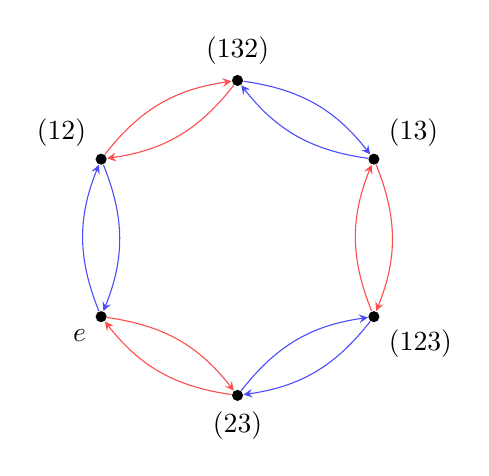
\begin{tikzpicture}
    \pgfmathsetmacro{\len}{2}
    \node[vertex,label=30:$(13)$]   (n13)  at (30:\len)  {};
    \node[vertex,label=90:$(132)$]  (n132) at (90:\len)  {};
    \node[vertex,label=150:$(12)$]  (n12)  at (150:\len) {};
    \node[vertex,label=210:$e$]     (ne)   at (210:\len) {};
    \node[vertex,label=270:$(23)$]  (n23)  at (270:\len) {};
    \node[vertex,label=330:$(123)$] (n123) at (330:\len) {};
    \begin{scope}[every to/.style={bend left=22}]
      % generator a is (12)
      \draw[gena] (ne)   to (n12);
      \draw[gena] (n12)  to (ne);
      \draw[gena] (n13)  to (n132);
      \draw[gena] (n132) to (n13);
      \draw[gena] (n123) to (n23);
      \draw[gena] (n23)  to (n123);
      % generator b is (23)
      \draw[genb] (ne)   to (n23);
      \draw[genb] (n23)  to (ne);
      \draw[genb] (n13)  to (n123);
      \draw[genb] (n123) to (n13);
      \draw[genb] (n12)  to (n132);
      \draw[genb] (n132) to (n12);
    \end{scope}
  \end{tikzpicture}
  \caption{Cayley diagram for $S_3$ with respect to $S = \{(12),(23)\}$.}
  \label{fig:cayley-s3}
\end{figure}

$G \equiv \Aut(D_G) \to \Sym(\Card G)$

\section{Actions}
\label{sec:actions}

If $G$ is any (possibly higher) group and $A$ is any type of objects,
then we define an \emph{action} by $G$ on an $A$ as a function
\[
  X : BG \to A.
\]
The particular $A$ being acted on is $X(\pt):A$,
and the action itself is given by transport.

Many times we are particularly interested in actions on types,
i.e., $A$ is a universe (or the universe of types-at-large):
\[
  X : BG \to \Type.
\]

In this case, we define \emph{orbit type} of the action as
\[
  X_G \defeq \sum_{z:BG} X(z),
\]
and the type of \emph{fixed points} as
\[
  X^G \defeq \prod_{z:BG} X(z).
\]
The set of orbits is the set-truncation of the orbit type,
\[
  X / G \defeq \Trunc{X_G}_0.
\]
We say that the action is \emph{transitive} if $X / G$ is contractible.

\section{Orbit-stabilizer theorem}
\label{sec:orbit-stabilizer-theorem}

Given an action $X : BG \to \Type$ and a point $x : X(\pt)$, we define
the \emph{orbit} through $x$ as the subtype of $X(\pt)$ consisting of
all $y : X(\pt)$ that are merely equal to $x$ in the orbit type:
\[
  G\cdot x \defeq \mathcal O_x \defeq \sum_{y : X(\pt)} \merely{[x] = [y]}
\]
(Note the unfortunate terminology: an orbit is not an element in the
orbit type!)
Note that this only depends on the image of $x$ in the set of orbits,
thus justifying the names.

In this way, the type $X(\pt)$ splits as a disjoint union of orbits,
indexed by the set of orbits
\[
  X(\pt) \equiv \coprod_{z : X / G} \mathcal O_z.
\]

The \emph{stabilizer group} $G_x$ of $x : X(\pt)$ is the automorphism group of $[x]$ in the orbit type.
Different points in the same orbit have conjugate stabilizer groups.

We say that the action is \emph{free} if all stabilizer groups are trivial.

\begin{theorem}[Orbit-stabilizer theorem]
  There is a canonical action $\tilde G : BG_x \to \Type$,
  acting on $\tilde G(\pt)\equiv G$
  with orbit type $\tilde G\dblslash G_x \equiv \mathcal O_x$.
\end{theorem}
\begin{proof}
  Define $\tilde G(x,y,!) \defeq (\pt = x)$.
\end{proof}

Now suppose that $G$ is a $1$-group acting on a set.
We see that the orbit type is a set
(and is thus equivalent to the set of orbits)
if and only if
all stabilizer groups are trivial,
\ie if and only if the action is free.

If $G$ is a $1$-group,
then so is each stabilizer-group,
and in this case (of a set-action),
the orbit-stabilizer theorem
tells us that 

\begin{theorem}[Lagrange's Theorem]
  If $H \to G$ is a subgroup, then $H$ has a natural action on $G$,
  and all the orbits under this action are equivalent.
\end{theorem}

% Interaction with cardinality: if G acts freely on S, then card(S/G) = card(S)/card(G)

\section{(the lemma that is not) Burnside's lemma}
\label{sec:burnsides-lemma}

% Where does this go?!
\section{More about automorphisms}
\label{sec:automorphisms}

% Written to record somewhere the results of a discussion with Bjorn
For every group $G$ (which for the purposes of the discussion
in this section we allow to be a higher group)
we have the automorphism group $\Aut(G)$.
This is of course the group of self-identifications $G = G$ in the type of groups, $\Group$.
If we represent $G$ by the pointed connected classifying type $BG$,
then $\Aut(G)$ is the type of pointed self-equivalences of $BG$.

We have a natural forgetful map from groups to the type of connected types.
Let $\Gerbe$ denote this type.
Thus, for every group $G$ we have a corresponding gerbe, $\gerbe(G)$.

\begin{definition}[The center as an abelian group]
  Let $Z(G) \defeq \prod_{z : BG}(z = z)$ denote the type of fixed points of the adjoint action of $G$ on itself.
  This type is equivalent to the automorphism group of the identity of $\gerbe(G)$,
  and hence the loop type of
  \[
    BZ(G) \defeq \sum_{f : BG \to BG} \merely{f \sim \id}.
  \]
  This type is itself the loop type of the pointed, connected type
  \[
    B^2Z(G) \defeq \sum_{X : \Gerbe}\Trunc{\gerbe(G) = X}_0,
  \]
  and we use this to give $Z(G)$ the structure of an \emph{abelian} group,
  called the \emph{center} of $G$.
\end{definition}
There is a canonical homomorphism from $Z(G)$ to $G$ given by the pointed map
from $BZ(G)$ to $BG$ that evaluates at the point $\pt$.
The fiber of the evaluation map $e : BZ(G) \to_\pt BG$ is
\begin{align*}
  \fiber_e(\pt)
  &\jdeq \sum_{f : BG \to BG} \merely{f \sim \id} \times (\mathop f \pt = \pt) \\
  &\equiv \sum_{f : BG \to_\pt BG} \merely{f \sim \id},
\end{align*}
and this type is the loop type of the pointed, connected type
\[
  \B\Inn(G) \defeq \sum_{H : \Group} \Trunc{\gerbe(G) = \gerbe(H)}_0,
\]
thus giving the homomorphism $Z(G)$ to $G$ a normal structure with
quotient group $\Inn(G)$, called the \emph{inner automorphism group}.

Note that there is a canonical homomorphism from $\Inn(G)$ to $\Aut(G)$
given by the pointed map $i : \B\Inn(G) \to \B\Aut(G)$ that forgets the component.
On loops, $i$ gives the inclusion into $\Aut(G)$ of the subtype of automorphisms of $G$
that become merely equal to the identity automorphism of $\gerbe(G)$.
The fiber of $i$ is
\begin{align*}
  \fiber_i(\pt)
  &\jdeq \sum_{H : \Group} \Trunc{\gerbe(G) = \gerbe(H)}_0 \times (H = G) \\
  &\equiv \Trunc{\gerbe(G) = \gerbe(G)}_0.
\end{align*}
This is evidently the type of loops in the pointed, connected $1$-type
\[
  \B\Out(G) \defeq \Trunc*{\sum_{X : \Gerbe}\merely{\gerbe(G) = X}}_1,
\]
thus giving the homomorphism $\Inn(G)$ to $\Aut(G)$ a normal structure with
quotient group $\Out(G)$, called the \emph{outer automorphism group}.
Note that $\Out(G)$ is always a $1$-group,
and that it is the decategorification of $\Aut(\gerbe(G))$.

\begin{theorem}
  Let two groups $G$ and $H$ be given.
  There is a canonical action of $\Inn(H)$
  on the set of homomorphisms from $G$ to $H$, $\Trunc{BG \to_\pt BH}_0$.
  This gives rise to an equivalence
  \[
    \Trunc{BG \to BH}_0 \equiv \Trunc*{\Trunc{BG \to_\pt BH}_0 \dblslash \Inn(H)}_0
  \]
  between the set of maps from $\gerbe(G)$ to $\gerbe(H)$ and the set of
  components of the orbit type of this action.
\end{theorem}
\begin{proof}
  We give the action by defining a type family $X : \B\Inn(H) \to \Type$ as follows
  \[
    X\, \angled{K,\phi} \defeq \Trunc{\Hom(G,K)}_0 \jdeq \Trunc{BG \to_\pt BK}_0,
  \]
  for $\angled{K,\phi} : \B\Inn(H) \jdeq \sum_{K : \Group} \Trunc{\gerbe(H) = \gerbe(K)}_0$.
  Now we can calculate
  \begin{align*}
    \Trunc{X_{\Inn(H)}}_0
    &\jdeq \Trunc*{\sum_{K:\Group}\Trunc{\gerbe(H)=\gerbe(K)}_0\times\Trunc{\Hom(G,K)}}_0 \\
    &\equiv \Trunc*{\sum_{K:\Group}(\gerbe(H)=\gerbe(K))\times\Hom(G,K)}_0 \\
    &\equiv \Trunc*{\sum_{K:\Gerbe}\sum_{k:K}(\gerbe(H)=K)\times\sum_{f:\Hom(\gerbe(G),K)}\mathop f \pt = k}_0 \\
    &\equiv \Trunc*{\sum_{K:\Gerbe} (\gerbe(H)=K) \times\Hom(\gerbe(G),K)}_0 \\
    &\equiv \Trunc*{\Hom(\gerbe(G),\gerbe(H))}_0 \jdeq \Trunc{BG \to BH}_0.\qedhere
  \end{align*}
\end{proof}

%%% Local Variables:
%%% mode: latex
%%% fill-column: 144
%%% TeX-master: "book"
%%% End:
